\documentclass[a4paper,12pt]{article}
\usepackage[a4paper,margin=2.4cm]{geometry} \linespread{1.25} 
\usepackage[english]{babel}

\usepackage{amsmath}
\usepackage{amssymb}
\usepackage[page,toc]{appendix}
\usepackage{fancyhdr}
\usepackage{fancyvrb}
\usepackage[T1]{fontenc}	
\usepackage{graphicx}
\usepackage[utf8]{inputenc}
\usepackage{titlesec}
\usepackage{hyperref}
\usepackage{enumitem}

\DeclareGraphicsExtensions{.png}	\graphicspath{{figures/}}               
\renewcommand{\arraystretch}{1.15}

\providecommand{\tightlist}{\setlength{\itemsep}{0pt}\setlength{\parskip}{0pt}}
% Needed for pandoc conversion

\fancyhf{}
\setlength{\headheight}{15pt}
\lfoot{}
\cfoot{}
\rfoot{\thepage{}}

\pagestyle{fancy}
\lhead{Group 12}
\chead{Compiler Construction - Final Report}
\rhead{\today}

\begin{document}

\begin{titlepage}

\newcommand{\HRule}{\rule{\linewidth}{0.5mm}}
% Defines a new command for 
% horizontal lines, change thickness here

\center % Centre everything on the page

	%------------------------------------------------
	%	Headings
	%------------------------------------------------

	\textsc{\LARGE University of Southern Denmark}\\[1.5cm]
	% Main heading such as the name of your university/college

	\textsc{\Large Department of Mathematics and Computer Science}\\[0.5cm]
	%Major heading such as course name

	\textsc{\large DM546: Compiler Construction}\\[0.5cm]
	% COURSE ID AND NAME

	%------------------------------------------------
	%	Title
	%------------------------------------------------

	\HRule\\[0.7cm]

	{\huge\bfseries Compiler Construction - Final Report}\\[0.4cm] % Title of your document

	\HRule\\[1.0cm]

	%------------------------------------------------
	%	Author(s)
	%------------------------------------------------
	\large
	\textsc{Authors:}\\ \bigskip
	\begin{minipage}[t]{0.45\textwidth}
	    \begin{center}
		    \normalsize
		    Nel Skowronek\\
		    nesko25@student.sdu.dk\\ \bigskip

	   \end{center}
	\end{minipage}
	~
	\begin{minipage}[t]{0.45\textwidth}
	    \begin{center}
		    \normalsize
		    Jan Ryszkiewicz\\
		    jarys25@student.sdu.dk\\ \bigskip
		\end{center}
	\end{minipage}
	

	%------------------------------------------------
	%	Date
	%------------------------------------------------

	\vfill\vfill\vfill % Position the date 3/4 down the remaining page

	{\large \today}

	%------------------------------------------------
	%	Logo
	%------------------------------------------------

	\vfill\vfill
	\begin{centering}
	
\includegraphics[width=0.3\textwidth]{SDU_logo}\\[1cm]
	% Include a 
% department/university logo - this will require the graphicx package
	\end{centering}
	
%-------------------------------------------------------------------------------

	\vfill % Push the date up 1/4 of the remaining page

\end{titlepage}

\section{Preliminaries}\label{preliminaries}

We implemented the interpreter using standard tools and libraries
available in Java. No parser generators or external frameworks were
used.

\section{Technical Description}\label{technical-description}

\subsection{Architecture}\label{architecture}

As shown below on the diagrams - the main class \texttt{VVPLController}
takes in the filepath of the file to interpret and:

\begin{enumerate}
\def\labelenumi{\arabic{enumi}.}
\tightlist
\item
  Runs the source code through the \texttt{Scanner} that generates
  tokens
\item
  Only when the \texttt{Scanner} succeeded - runs the tokens through the
  \texttt{Parser} that generates the Abstract Syntax Tree (it's basic
  parent node being \texttt{Declaration})
\item
  Only when the \texttt{Parser} succeeded - runs the
  \texttt{Declaration}s (AST) through the Semantic Checker (called
  \texttt{Canary} here, because it checks everything at once before the
  final evaluation - like the bird)
\item
  And finally, only when \texttt{Canary} succeeded - runs the
  \texttt{Interpreter} on the AST
\end{enumerate}

If at any point in this chain of execution an error appears - the static
\texttt{ErrorHandler} class is used to store all the errors and print
them all at the end of a phase (eg. during parsing) to allow the program
to check for all the error in that phase, not just the first encountered
one. This is also visible on the activity diagram below. \newline

\subsubsection{Class Diagram}\label{class-diagram}

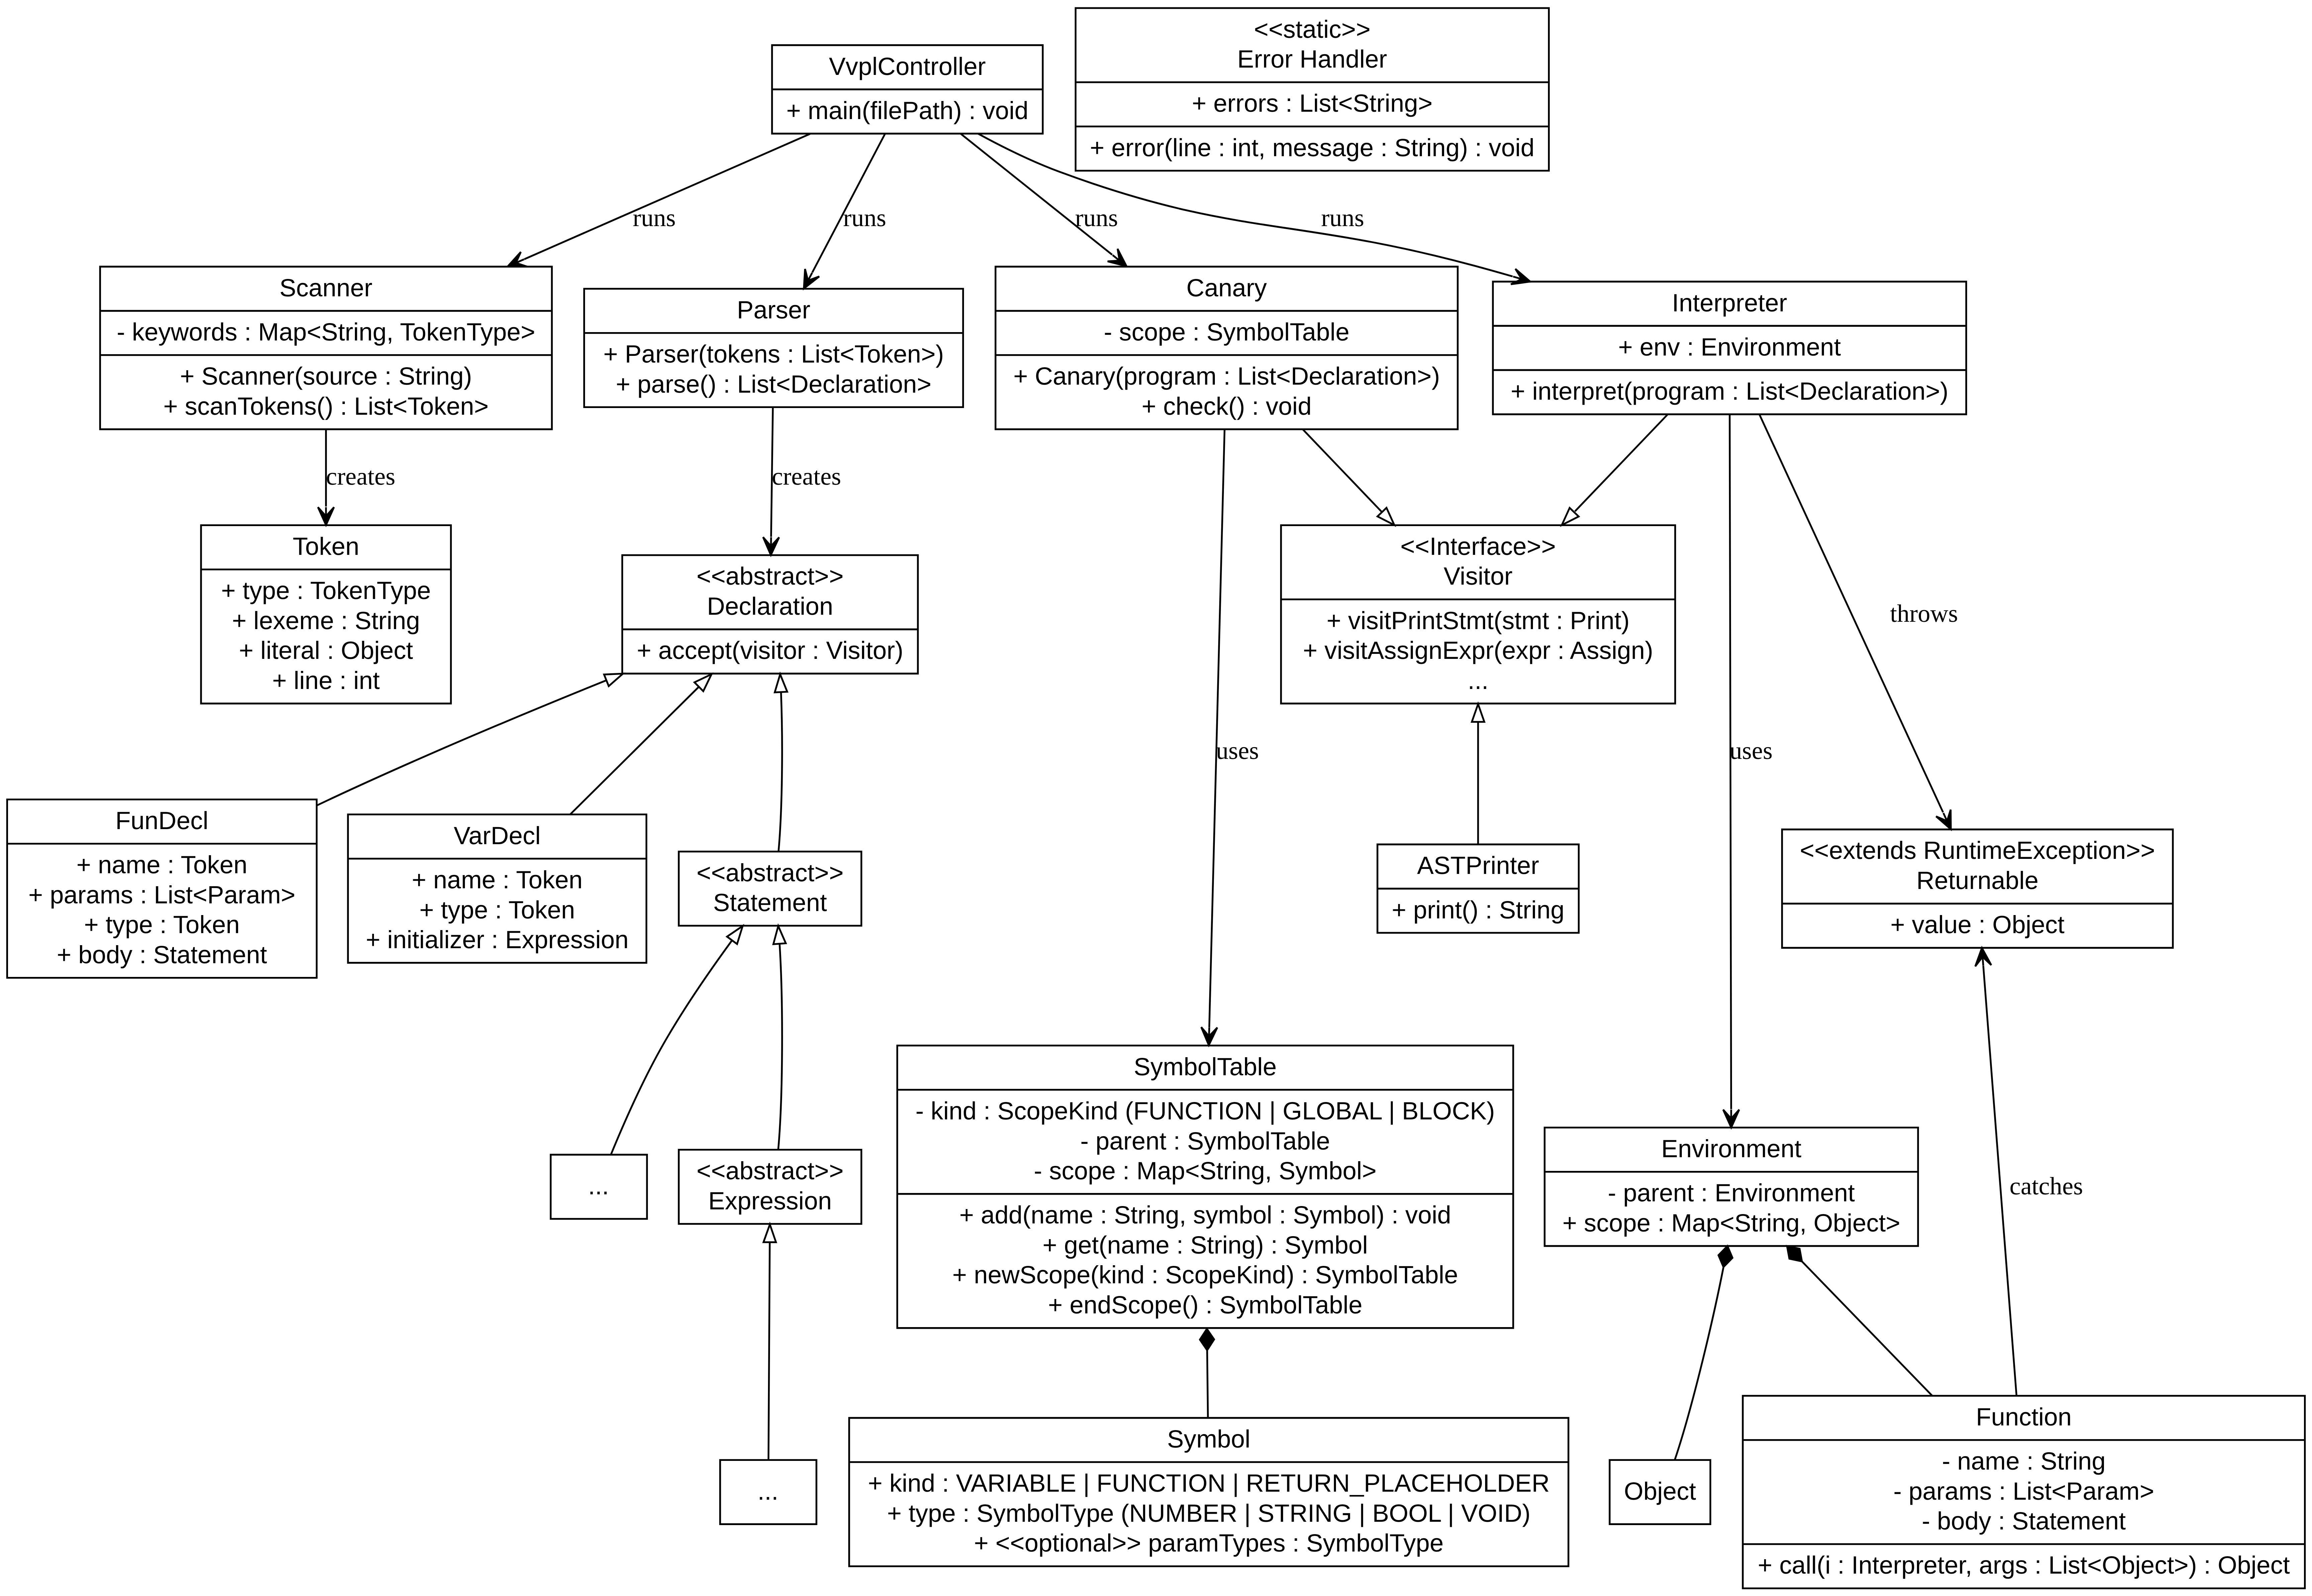
\includegraphics[width=6in,height=4.5in]{report_files/figure-latex/dot-figure-1.png}

\subsubsection{Activity Diagram}\label{activity-diagram}

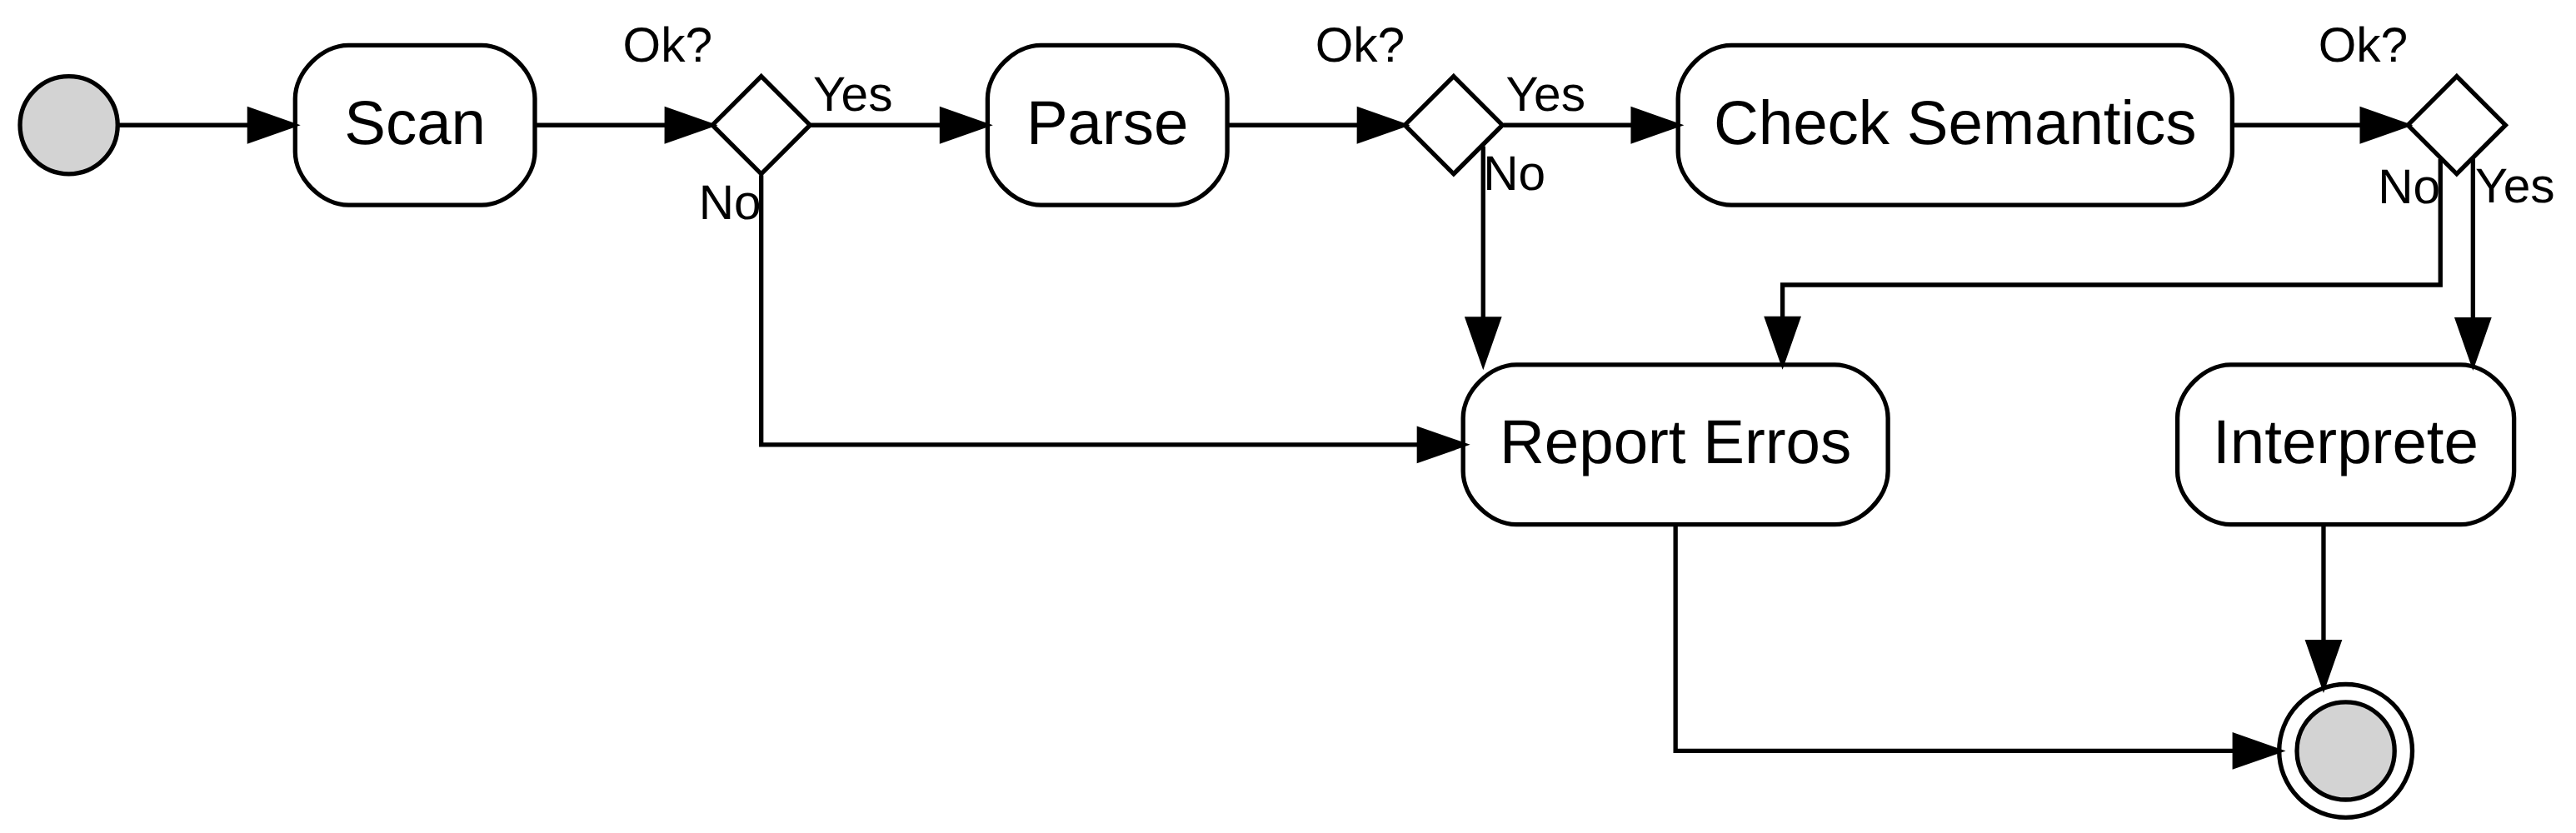
\includegraphics[width=6in,height=2in]{report_files/figure-latex/dot-figure-2.png}

This clear division of phases allows the code to be Single-Resposibility
and Open-Close as it makes it very easy to change how one phase is
executed, or to insert an additional phase at any point - without
influencing other classes. \newline

Additionally the Visitor Pattern was used to visit the AST nodes, which
keeps the implementation of the nodes clean and focused only on their
data - allowing for easy implementation of the Semantic Checker, the
Tree-Walk \texttt{Interpreter}, the \texttt{ASTPrinter} (for debugging
purposes) and possible additional checkers if need be.

\subsection{Implementation}\label{implementation}

\subsubsection{Scanning}\label{scanning}

The \texttt{Scanner} goes through the source code character-by-character
and handles each expected character in it's respective way via a simple
switch-case. It matches single-character tokens right away, and for
single or 2-character tokens (eg. `\textless{}' could be either
`\textless{}' or `\textless=') it looks one character ahead. For longer
and more complicated tokens (such as ids, keywords, literal strings and
numbers) it reads all expected characters until a specified end (usually
a whitespace or a quotation mark) and checks via a hash-map if the
resulting lexeme is a keyword or not. \newline

All whitespaces (except in strings) are ignored, and all unexpected
characters result in a \texttt{ScanError}.

\subsubsection{Parsing}\label{parsing}

We implemented a recursive-descent \texttt{Parser} with one lookahead.
It implements the production rules as specified in the grammar by
calling an appropriate recursive method for each rule (eg.
\texttt{declaration()}, \texttt{ifStmt()}, \texttt{or()}\ldots). All
ambiguities are resolved by looking one token ahead and matching it with
a production rule. All unexpected tokens that don't match any of the
production rules result in a \texttt{ParseError}. At this point the
\texttt{Parser} skips to the next semicolon token to ``synchronize'' to
the next declaration. \newline

For the \texttt{cast} expression a specific class for the AST was
defined that has two children: \texttt{type} (leaf) and \texttt{value}
(deriving from \texttt{expression}). This allows for very easy
type-checking and interpreting of cast expressions as well as nested
\texttt{cast} expressions. \newline

The ``dangling else'' is assigned to \textbf{the most nested if}, and
all following ``elses'' are assigned to the second most nested, the
third, and so on.

\subsubsection{Semantic Analysis}\label{semantic-analysis}

We perform the Scope Analysis and Type Analysis simultaneously, due to
their similar nature and to avoid overhead of running the checker twice.
But first we quickly go over the list of declarations and add the
signatures of function declarations as \texttt{Symbol}s to the
\texttt{SymbolTable} to allow for out-of-order declarations of functions
in the global scope. Then we properly walk the tree and for every AST
node we check the applicable properties:

\begin{itemize}
\tightlist
\item
  if a variable has been defined (we don't allow shadowing)
\item
  if a function has been defined
\item
  if a function is not being defined anywhere other than the global
  scope
\item
  if function parameters have unique names
\item
  if there is no unreachable code after a \texttt{return} statement
\item
  if there is no return statement outside a function
\end{itemize}

And for each AST node, if none of the above applicable properties were
violated, we check:

\begin{itemize}
\tightlist
\item
  if the initializer type matches the declared variable type
\item
  if there is an initializer at all
\item
  if binary operands are of correct type
\item
  if logical operands are of correct type
\item
  if a value can be casted
\item
  if the type of returned value matches the declared function type
\end{itemize}

To do that, the Semantic Check \texttt{Visitor} returns a
\texttt{SymbolType} when visiting any node, to pass information to the
parent node about it's children's types. All declarations are stored in
the \texttt{SymbolTable} and a new \texttt{SymbolTable} is created for
each block or function and then destroyed at the end of the scope,
disallowing the usage of variables defined in a deeper scope. \newline

To handle the return statements, at the beginning of
\texttt{visitFunDecl()} method a special symbol is added to the
function's \texttt{SymbolTable} that acts as a placeholder for the
return value and stores information about it's expected type. While
visiting the \texttt{returnStmt} the checker can then check if the
current scope is a function scope (it keeps that information) and
extract the special symbol's type to compare it with the statement's
\texttt{value} child node's type. \newline

If a function's type is unspecified it is treated as \texttt{void}-type
and all return statements in that function are expected to not have a
value. \newline

If any properties are violated the checker (similarly to
\texttt{Scanner} and \texttt{Parser}) reports either a
\texttt{ScopeError} or a \texttt{TypeError} to the
\texttt{ErrorHandler}, and returns \texttt{null} as the type of the
node. That way parent nodes know that something went wrong and can keep
on looking for different violations, instead of propagating the same
error higher.

\subsubsection{Interpretation}\label{interpretation}

As mentioned before, the \texttt{Interpreter} is an AST \texttt{Visitor}
and executes the code by walking the tree. It assumes that everything
that ought to have been checked during previous phases has been checked
correctly and that no error appeared along the way. \newline

That being said, the \texttt{Interpreter} is still checking for a few
things:

\begin{itemize}
\tightlist
\item
  division by 0
\item
  runtime evaluable casting rules (what boolean value to cast a number
  to, and if a string can be casted to a number)
\end{itemize}

And throws a \texttt{RuntimeError} and stops the execution if need be.
\newline

An \texttt{Environment} is used to map variable names to objects with
their value at any given moment. Additionally, to handle functions, a
new \texttt{Function} class has been declared (also mapped in the
environment to the function name), that stores the function's
declaration's AST node and interprets it (using the same interpreter,
but a new, local environment) everytime it is called. The local
environment initially contains only the mapping of parameter names (here
we're allowing shadowing global variables) onto their respective values,
given by the \texttt{callExpr}, and other globally declared functions.
\newline

Function class itself, when called, binds all arguments, copies current
interpreter environment, flags etc. to be later retreived and creates a
fresh environment for the interpreter with needed function declarations
and variables that then runs the function in
\texttt{inFunction\ =\ true} mode expecting a return value (if void,
returns null). After function is evaluated it returns the interpreter to
the state before function call, and sets the \texttt{inFunction} flag to
false. This method allows reusage of existing instance of the
interpreter and avoids recursive creation of new ones when calling a big
recursive function (reduces stack usage). \newline

The returns themselves are handled by \texttt{visitReturnStmt()} method
that throws a special kind of error - \texttt{Returnable} - that
remembers the value object that is being returned. That
\texttt{Returnable} error is then caught by the mentioned above
\texttt{Function} object. The returned value is extracted and returned
back to the initial \texttt{callExpr}.

\subsubsection{Monitoring and Logging}\label{monitoring-and-logging}

Due to the clear phase division, it is easy to add logging (printing the
tokens or the AST) at any point of the interpretation process. However,
we don't do that during the main program execution - the only things
that appear is the output of the program, or the errors. The logging is
used only for certain tests.

\subsection{Testing \& Evaluation}\label{testing-evaluation}

We created convenient test classes that dynamically create unit tests
for all files in their respective \texttt{resources} directory. They run
the tested component on the given \texttt{.in} file and compare the
results with the given \texttt{.\textless{}component\textgreater{}} or
\texttt{.out} file. We tried to test all major components, all AST nodes
and almost all errors that are possible to appear. \newline

The only thing we changed in the given tests was the way the errors were
printed and their content - to align with our errors which we tried to
make more descriptive. We made sure that that the error types and lines
were identical.

\section{Teamwork Organization}\label{teamwork-organization}

As our team consists of 2 people and there are 4 major components/phases
of our interpretation process - each person worked on 2 of the
components.

\begin{itemize}
\tightlist
\item
  \textbf{Nel}: Parsing and Semantic Checks
\item
  \textbf{Jan}: Scanning and Interpreting
\end{itemize}

This division allowed to avoid potential merge-conflicts. Our workflow
was organized through Git and we communicated regularly to ensure
consistency in error handling and the interpretation pipeline itself.
\newline

While we were already familiar with regexes, we definitely learned a lot
about finite automatas, grammars, production rules, IRs - but mostly
about LL(1) grammars of course, since that was the grammar of the
language we were interpreting.

\section{Discussion}\label{discussion}

Alternatively to writing the scanner and the parser ourselves, we
could've used various scanner and parser generators (like Flex and Bison
for C) which could guarantee correctness, save time and work and teach
us how to use a new framework. On the other hand, the downside of this
option is that possibly, we would have to spend more time learning to
use this technology and later it might have prove inefficient and a
slight overkill for such a small language. \newline

At this point adding anything new to the language and grammar would
require substantial changes in each and every part of our program.
Automation of Scanners and Parsers and more unified way of handling AST
could be helpful if we ever decided to expand the VVPL. \newline

Using Tree-Walk interpreter is also considered very inefficient, it'd be
better to first translate the code into more LLVM-like structure and
then run the ByteCode itself as it has a lot of built in optimizations
we wouldn't have to worry about. Using try-catch methods as a way of
returing functions also introduces a lot of overhead. \newline

Overall, changing the general form of the interpreter and automating the
Scanner and Parser could allow us to create a bigger, faster and easier
to modify language (compiled into LLVM, then either interpreted or
compiled to Machine Code using \textbf{clang}). Possible new features
would include allowing user inputs or explicit memory allocation.

\end{document}
